\chapter{影子与日食}\label{ch:g7:shadows-eclipses}

一生中有那么一两次，在短短几分钟里，白昼变成了黑夜：
太阳的圆面被\omterm{def:g2:moon-in-the-sky:moon}{月球}遮住，正午时分竟能看到星星。
古人从中读出了灾祸的预兆，而你将读出的是几何。
\omterm{def:g7:shadows-eclipses:solar}{日食}不过是一个\omterm{def:g1:light-and-shadows:shadow}{影子}——是你一生中会站进去的最大的\omterm{def:g1:light-and-shadows:shadow}{影子}——
而你的直尺与\omterm{def:g6:light-propagation:ray}{光线}工具箱，
正是它所遵循的规律。

\section{来自“理想”光源的影子}

\begin{proposition}[本影与半影]\label{prop:g7:shadows-eclipses:umbra}
\emph{点状}\omterm{def:g1:light-and-shadows:source}{光源}投射出一个边缘清晰的单一\omterm{def:g1:light-and-shadows:shadow}{影子}。
\emph{宽大}\omterm{def:g1:light-and-shadows:source}{光源}——如磨砂灯罩，或太阳的整个圆面——
投射出由两部分组成的\omterm{def:g1:light-and-shadows:shadow}{影子}：
\begin{enumerate}
  \item \emph{本影}\index{本影}：被\omterm{def:g1:light-and-shadows:source}{光源}
        \emph{任何部分}发出的光都照不到的区域——完全
        黑暗；
  \item \emph{半影}\index{半影}：边缘区域，只受\omterm{def:g1:light-and-shadows:source}{光源}
        \emph{某一部分}发出的光所照到的区域——半明半暗，
        并向外逐渐变淡。
\end{enumerate}
在\omterm{prop:g7:shadows-eclipses:umbra}{本影}之内，\omterm{def:g1:light-and-shadows:source}{光源}被完全遮住；在
\omterm{prop:g7:shadows-eclipses:umbra}{半影}之内，\omterm{def:g1:light-and-shadows:source}{光源}仅被部分遮住——从遮挡物边缘“探出”一点。
\end{proposition}

\begin{method}[作出两种影子]\label{met:g7:shadows-eclipses:construct}
对于宽大\omterm{def:g1:light-and-shadows:source}{光源}，决定\omterm{def:g1:light-and-shadows:shadow}{影子}分布的是其\emph{边缘}发出的\omterm{def:g6:light-propagation:ray}{光线}：
\begin{enumerate}
  \item 从\omterm{def:g1:light-and-shadows:source}{光源}上边缘出发，画出擦过遮挡物两侧的\omterm{def:g6:light-propagation:ray}{光线}，
        再以同样方法从下边缘画出。
  \item 遮挡物后方，\emph{两}条边缘的\omterm{def:g6:light-propagation:ray}{光线}都照不到的区域，
        即为\omterm{prop:g7:shadows-eclipses:umbra}{本影}；
  \item 只被一条边缘的\omterm{def:g6:light-propagation:ray}{光线}照不到、而被另一条
        边缘的\omterm{def:g6:light-propagation:ray}{光线}照到的两侧区域，即为\omterm{prop:g7:shadows-eclipses:umbra}{半影}；
  \item 所有\omterm{def:g6:light-propagation:ray}{光线}都能到达之处，即为全亮。
\end{enumerate}
圆形遮挡物的\omterm{prop:g7:shadows-eclipses:umbra}{本影}是一个圆锥——而这个圆锥能否
到达某个屏幕，决定了\omterm{def:g7:shadows-eclipses:solar}{日食}的一切。
\end{method}

\begin{omfigure}
\begin{tikzpicture}[scale=0.8]
  \draw[thick, fill=omThm, fill opacity=0.4] (0.5,1.1) circle (0.55);
  \node[below, font=\small] at (0.5,0.3) {宽大光源};
  \draw[thick, fill=omDef, fill opacity=0.4] (4.3,1.1) circle (0.42);
  \draw[very thick] (10.6,-1.3) -- (10.6,3.5);
  \draw[omThm] (0.5,1.65) -- (4.55,1.42) -- (10.6,0.52);
  \draw[omThm] (0.5,1.65) -- (4.05,0.78) -- (10.6,-0.9);
  \draw[omThm] (0.5,0.55) -- (4.55,0.78) -- (10.6,1.68);
  \draw[omThm] (0.5,0.55) -- (4.05,1.42) -- (10.6,3.1);
  \draw[line width=3.5pt, omExo] (10.6,0.52) -- (10.6,1.68);
  \draw[line width=3.5pt, omExo, opacity=0.45]
    (10.6,-0.9) -- (10.6,0.52);
  \draw[line width=3.5pt, omExo, opacity=0.45]
    (10.6,1.68) -- (10.6,3.1);
  \node[right, font=\small] at (10.75,1.1) {本影};
  \node[right, font=\small] at (10.75,2.5) {半影};
  \node[right, font=\small] at (10.75,-0.3) {半影};
\end{tikzpicture}

{\small 宽大\omterm{def:g1:light-and-shadows:source}{光源}的双层\omterm{def:g1:light-and-shadows:shadow}{影子}：\omterm{prop:g7:shadows-eclipses:umbra}{本影}处完全看不到\omterm{def:g1:light-and-shadows:source}{光源}；
\omterm{prop:g7:shadows-eclipses:umbra}{半影}处只看不到\omterm{def:g1:light-and-shadows:source}{光源}的一部分。}
\end{omfigure}

\begin{example}[处处都是柔和的边缘]\label{ex:g7:shadows-eclipses:soft}
现在，磨砂灯与阴天所造成的模糊\omterm{def:g1:light-and-shadows:shadow}{影子}也都可以解释了：
宽大\omterm{def:g1:light-and-shadows:source}{光源}使每个\omterm{def:g1:light-and-shadows:shadow}{影子}都带上\omterm{prop:g7:shadows-eclipses:umbra}{半影}，
而足够大的\omterm{def:g1:light-and-shadows:source}{光源}（如整片阴云密布的天空）所产生的几乎全是\omterm{prop:g7:shadows-eclipses:umbra}{半影}——
\omterm{def:g1:light-and-shadows:shadow}{影子}被冲淡至几乎消失。你正午时分的\omterm{def:g1:light-and-shadows:shadow}{影子}边缘，
细看之下是一条宽约一\omterm{def:g2:measuring-length:units}{厘米}的柔和\omterm{prop:g7:shadows-eclipses:umbra}{半影}带：太阳
是一个圆面而不是一个点，这条\omterm{prop:g7:shadows-eclipses:umbra}{半影}带正是它的“自白”。
\end{example}

\section{月球走进光束}

\begin{definition}[日食]\label{def:g7:shadows-eclipses:solar}
\emph{日食}\index{日食}发生时，\omterm{def:g2:moon-in-the-sky:moon}{月球}恰好
位于太阳与地球之间，其\omterm{def:g1:light-and-shadows:shadow}{影子}落下，
落到地球上。\omterm{def:g2:moon-in-the-sky:moon}{月球}的\emph{\omterm{prop:g7:shadows-eclipses:umbra}{本影}}触及地球处——一个移动迅速的光斑，
宽度往往只有两百千米左右——太阳的圆面
被完全遮住，形成\emph{全}食：白昼变成黑夜，
星星显现。在周围广阔的\emph{\omterm{prop:g7:shadows-eclipses:umbra}{半影}}区域，太阳
只是部分被遮住，形成\emph{偏}食。
\end{definition}

\begin{definition}[月食]\label{def:g7:shadows-eclipses:lunar}
\emph{月食}\index{月食}发生时，
\emph{\omterm{def:g2:moon-in-the-sky:moon}{月球}}进入\emph{地球}的影锥时，\omterm{ex:g2:moon-in-the-sky:shapes}{满月}
变暗——常常呈现深铜色的光辉——持续
一\omterm{ex:g2:measuring-time:clock}{小时}或更久，整个夜半球的人都能同时看到。这
一次，我们是遮挡物，\omterm{def:g2:moon-in-the-sky:moon}{月球}则处在我们的\omterm{prop:g7:shadows-eclipses:umbra}{本影}之中。
\end{definition}

\begin{omfigure}
\begin{tikzpicture}[scale=0.8]
  \draw[thick, fill=omThm, fill opacity=0.4] (0.6,1.2) circle (0.7);
  \node[below, font=\small] at (0.6,0.2) {太阳};
  \draw[thick, fill=omExo, fill opacity=0.6] (5.4,1.2) circle (0.16);
  \node[above, font=\small] at (5.4,1.55) {月球};
  \draw[thick, fill=omDef, fill opacity=0.4] (9.4,1.2) circle (0.55);
  \node[below, font=\small] at (9.4,0.35) {地球};
  \draw[omThm] (0.6,1.9) -- (5.4,1.36) -- (8.88,1.28);
  \draw[omThm] (0.6,0.5) -- (5.4,1.04) -- (8.88,1.12);
  \fill[omExo] (8.86,1.2) circle (0.07);
  \node[right, font=\footnotesize] at (9.9,1.85)
    {本影的尖端：一个小小的移动光斑};
  \draw[-Stealth, omExo] (9.9,1.75) -- (8.98,1.3);
\end{tikzpicture}

{\small \omterm{def:g7:shadows-eclipses:solar}{日食}几何关系（大小和间距严重失真，
不成比例）：\omterm{def:g2:moon-in-the-sky:moon}{月球}细长的\omterm{prop:g7:shadows-eclipses:umbra}{本影}恰好触及地球——
处于其尖端之下的幸运地点即可看到全食。}
\end{omfigure}

\begin{example}[为何如此罕见？]\label{ex:g7:shadows-eclipses:rare}
每个月都有新月，为何不每个月都有\omterm{def:g7:shadows-eclipses:solar}{日食}？
因为\omterm{def:g2:moon-in-the-sky:moon}{月球}\omterm{def:g6:sun-earth-moon:axisorbit}{轨道}相对地球绕日路径\emph{倾斜}，
倾角约为五度。大多数月份里，
新月会从太阳–地球连线的\emph{上方}或\emph{下方}经过，
其\omterm{def:g1:light-and-shadows:shadow}{影子}无害地射向太空。只有当新月
恰好在\omterm{def:g2:moon-in-the-sky:moon}{月球}穿越排列面时出现，
三个天体才会排成一线——每年地球上某处会有数次，
但对任一\emph{特定}城镇而言，全食是
一生难得一遇的访客。
\end{example}

\begin{omfigure}
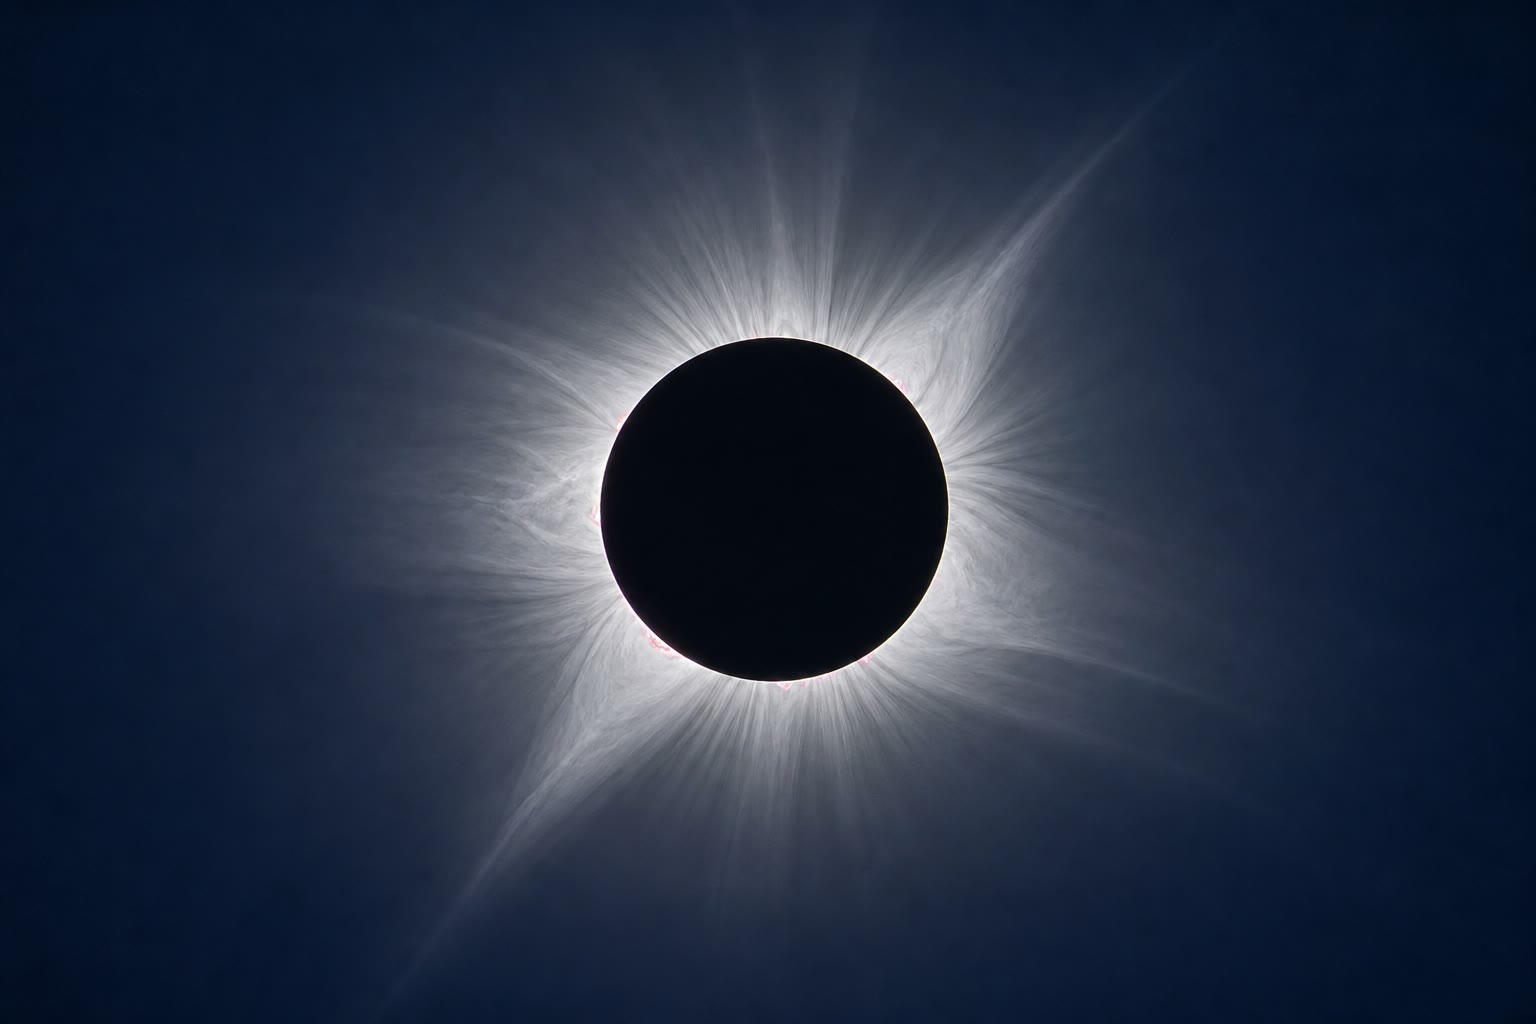
\includegraphics[width=0.55\linewidth]{images/book1/ai/g7-eclipse-corona.jpg}

{\small 全食：\omterm{def:g2:moon-in-the-sky:moon}{月球}圆面恰好遮住太阳圆面，几分钟内可以看到日冕——即太阳的外层大气——环绕在黑色圆面周围。}
\end{omfigure}

\begin{example}[造成全食的巧合]\label{ex:g7:shadows-eclipses:coincidence}
你的操场模型已经发现了：太阳比\omterm{def:g2:moon-in-the-sky:moon}{月球}约宽 $400$ 倍，
而且距离地球也约远 $400$ 倍。
因此两者在天空中的视圆面几乎完全吻合，所以
\omterm{def:g2:moon-in-the-sky:moon}{月球}\emph{刚好}能遮住太阳：全食时间短暂，
\omterm{prop:g7:shadows-eclipses:umbra}{本影}光斑很小。当\omterm{def:g2:moon-in-the-sky:moon}{月球}位于其略呈椭圆的\omterm{def:g6:sun-earth-moon:axisorbit}{轨道}
远端时，其圆面不足以遮住太阳，一圈炽亮的
太阳边缘环绕着黑色的\omterm{def:g2:moon-in-the-sky:moon}{月球}——即\emph{环食}，
美丽却不加防护地观看绝不安全。
\end{example}

\begin{remark}[观日而不伤目]\label{rem:g7:shadows-eclipses:safety}
古老规则对\omterm{def:g7:shadows-eclipses:solar}{日食}也不例外：\emph{绝不}
直视太阳——无论\omterm{def:g7:shadows-eclipses:solar}{日食}与否——也不可用肉眼、
墨镜或任何透镜。被部分遮挡的太阳灼伤视网膜的力度，
与完整的太阳同样严重，而且毫无痛感。
安全的观测工具都是老朋友：针孔——将太阳的像
通过一个小孔投射到纸上，舒适地看着缺口逐渐变大——
或一棵树叶茂密的树，其上千个叶间缝隙形成的针孔，
在地面上洒满细小的月牙。只有经过认证的\omterm{def:g7:shadows-eclipses:solar}{日食}眼镜，
经检验且完好无损者，才可直接面对太阳；在
\emph{全食}的短短几分钟内，可以裸眼欣赏日冕，
但第一缕重现的日光一出现，这份休战便告结束。
\end{remark}

\section{练习}

\begin{exercise}[$\star$]\label{exo:g7:shadows-eclipses:1}
试根据位于\omterm{prop:g7:shadows-eclipses:umbra}{本影}或\omterm{prop:g7:shadows-eclipses:umbra}{半影}内的眼睛能看到\omterm{def:g1:light-and-shadows:source}{光源}的
哪一部分，分别定义\omterm{prop:g7:shadows-eclipses:umbra}{本影}与\omterm{prop:g7:shadows-eclipses:umbra}{半影}。
\end{exercise}

\begin{exercise}[$\star$]\label{exo:g7:shadows-eclipses:2}
为何点状\omterm{def:g3:first-electric-circuit:bulb}{灯泡}完全不会投下\omterm{prop:g7:shadows-eclipses:umbra}{半影}？又为何
阴天时几乎不产生\omterm{def:g1:light-and-shadows:shadow}{影子}，这又是为何？
\end{exercise}

\begin{exercise}[$\star$]\label{exo:g7:shadows-eclipses:3}
在作图法中，哪些\omterm{def:g6:light-propagation:ray}{光线}描绘出\omterm{def:g1:light-and-shadows:shadow}{影子}的轮廓——
是\omterm{def:g1:light-and-shadows:source}{光源}的中心还是边缘发出的\omterm{def:g6:light-propagation:ray}{光线}？什么标出了\omterm{prop:g7:shadows-eclipses:umbra}{本影}？
\end{exercise}

\begin{exercise}[$\star$]\label{exo:g7:shadows-eclipses:4}
\omterm{def:g7:shadows-eclipses:solar}{日食}：将太阳、\omterm{def:g2:moon-in-the-sky:moon}{月球}和地球按顺序排列，并说明
当天\omterm{def:g2:moon-in-the-sky:moon}{月球}应处于何种月相。\omterm{def:g7:shadows-eclipses:lunar}{月食}：提出
同样的两个问题。
\end{exercise}

\begin{exercise}[$\star$]\label{exo:g7:shadows-eclipses:5}
\omterm{def:g7:shadows-eclipses:solar}{日食}期间，谁能看到全食，谁能看到
部分遮挡，谁又完全看不出任何异常？
\end{exercise}

\begin{exercise}[$\star$]\label{exo:g7:shadows-eclipses:6}
为何\omterm{def:g7:shadows-eclipses:lunar}{月食}能同时在半个地球上看到，
而全食的路径却是一条狭窄、飞速移动的条带？
\end{exercise}

\begin{exercise}[$\star$]\label{exo:g7:shadows-eclipses:7}
尽管每个月都有新月和\omterm{ex:g2:moon-in-the-sky:shapes}{满月}，为何并非每月都有
\omterm{def:g7:shadows-eclipses:solar}{日食}或\omterm{def:g7:shadows-eclipses:lunar}{月食}？
\end{exercise}

\begin{exercise}[$\star$]\label{exo:g7:shadows-eclipses:8}
列举两种观察\omterm{def:g7:shadows-eclipses:solar}{日食}进程的安全方法，以及
允许裸眼观看的那一刻。
\end{exercise}

\begin{exercise}[$\star\star$]\label{exo:g7:shadows-eclipses:9}
解释 $400$ 与 $400$ 的巧合及其两个
后果：全食的近乎完美吻合，以及
环食中的光环。
\end{exercise}

\begin{exercise}[$\star\star$]\label{exo:g7:shadows-eclipses:10}
仔细观察正午时自己\omterm{def:g1:light-and-shadows:shadow}{影子}的边缘：脚下清晰，
头部的\omterm{def:g1:light-and-shadows:shadow}{影子}边缘则较为模糊。请用太阳圆面和作图法
解释这种渐变——为何\omterm{prop:g7:shadows-eclipses:umbra}{半影}
随着离遮挡物的距离增大而变宽？
\end{exercise}

\begin{exercise}[$\star\star$]\label{exo:g7:shadows-eclipses:11}
在\omterm{def:g7:shadows-eclipses:solar}{日食}部分遮挡期间，两年前的那些树叶
月牙又出现了。请完整解释它们：每个叶隙是
什么，每个地面光斑是什么，
为何所有月牙都朝同一方向？
\end{exercise}

\begin{exercise}[$\star\star\star$]\label{exo:g7:shadows-eclipses:12}
在\emph{月}全食期间，\omterm{def:g2:moon-in-the-sky:moon}{月球}很少完全消失：它
呈深铜红色。到达\omterm{def:g2:moon-in-the-sky:moon}{月球}的\omterm{def:g6:light-propagation:ray}{光线}已擦过地球的
边缘——穿过环绕地球的\omterm{def:g1:day-and-night:daynight}{日落}时分的大气，
同时穿过整个地球。请用上一章的长程漫射，
拼出完整解释：大气对擦过的光做了什么，
为何幸存的光是红色？（你要一次说清，
为何被遮的\omterm{def:g2:moon-in-the-sky:moon}{月球}会带上地球上
每次\omterm{def:g1:day-and-night:daynight}{日落}的颜色。）
\end{exercise}

\section{问题：日食考察}

\begin{problem}[{周末问题——班级规划日食考察：
几何选营地，物理装行囊；
全食时刻，逐分钟}]\label{pb:g7:shadows-eclipses:1}
明年春天，一次日全食横穿这片大陆。
全班将规划一次考察——用\omterm{def:g6:light-propagation:ray}{光线}图，而非宣传册。

\medskip\noindent\textbf{第一部分——选择站位。}
地图集给出预测路径：一条宽 \qty{160}{km} 的条带
横穿地图，两侧是偏食区，
其宽度达数千千米。
\begin{enumerate}
  \item 该条带划定的是哪种影区，
        其两侧又是哪一区域？
  \item 全班所在的小镇位于距条带中线 \qty{300}{km} 处，
        \omterm{def:g7:shadows-eclipses:solar}{日食}当天小镇将看到什么？
  \item 考察队为何必须前往该条带——
        “在家看到百分之九十五的偏食”为何无法
        在正午显出夜色、星星或日冕？
  \item 条带预报标注全食于 10:41 出现，
        在中线处持续 $3$ 分 $12$ 秒，
        向两侧则更短。为何全食
        在条带中心时最长？
\end{enumerate}

\medskip\noindent\textbf{第二部分——准备物理装备。}
\begin{enumerate}[resume]
  \item 老师带上了合格的\omterm{def:g7:shadows-eclipses:solar}{日食}观测眼镜，并没收
        两副太阳镜。请说明这两种做法的理由。
  \item 每位学生都要用一个鞋盒制作针孔
        投影仪。回想其结构，并说明
        应相对太阳朝哪个方向站立。
  \item 有学生提议“在一桶水的\omterm{def:g5:mirrors-reflection:reflection}{反射}里观看
        ”。请对这一提议作出裁定。
  \item 小组还将携带一个漏勺，举在一张
        白纸上方。预测并解释其数十个
        孔洞在偏食阶段会投下什么图样。
\end{enumerate}

\medskip\noindent\textbf{第三部分——当天的情况，逐
分钟推进。}
\begin{enumerate}[resume]
  \item 09:30，初亏：透过眼镜，太阳边缘出现一小块
        缺口。遮挡太阳的是什么天体，
        它的哪一种影区已到达
        营地？
  \item 10:39：\omterm{def:g6:light-propagation:ray}{光线}变得诡异而昏暗；地面上的
        \omterm{def:g1:light-and-shadows:shadow}{影子}边缘异常清晰。请用\omterm{prop:g7:shadows-eclipses:umbra}{本影}与\omterm{prop:g7:shadows-eclipses:umbra}{半影}的
        思路解释这种变清晰的原因——
        随着太阳可见的细弧变窄，太阳正在变成什么？
  \item 10:41，全食：按规定摘下眼镜。在 $3$
        分钟内，全班站在某种东西之中。请准确说出其名称，
        并说明黑色圆盘周围变得可见的是什么——
        以及为何“休战”恰在第一道
        返回的细弧出现时结束？
  \item 12:00，在回家的大巴上，老师请大家给出
        一句话总结：“\omterm{def:g7:shadows-eclipses:solar}{日食}是\dots”。请把它补充完整，
        让其中包含本章的几何内容。
\end{enumerate}
\end{problem}
